\documentclass{svjour3}  
\RequirePackage{fix-cm}
\usepackage{nicefrac}
\usepackage{graphicx}
\usepackage{lineno}
\usepackage{natbib} 
\usepackage{geometry}
\usepackage{pdflscape}
\usepackage{setspace,caption}
\renewcommand{\familydefault}{\sfdefault}
\usepackage{epigrafica}
\usepackage[LGR, T1]{fontenc}
% Tables 
	\usepackage{booktabs}
	\usepackage{enumitem}
	\usepackage{array}
	
	\usepackage{makecell,
		multirow}
	\renewcommand\theadfont{\bfseries\normalsize}
	
	\newcommand{\tablistcommand}{% 
		\leavevmode\par\vspace{-\baselineskip}
	}

\captionsetup{font=doublespacing}% Double-spaced float captions

\doublespacing% Double-spaced document text

\usepackage[pdfpagelabels=true,plainpages=false,colorlinks=true,
    linkcolor=blue,citecolor=blue,urlcolor=blue]{hyperref}

\journalname{Plant Ecology}

\begin{document}
	\linenumbers
	
	\title{Fugitive road dust alters annual plant physiology but perennial grass growth appears resistant}
	
	\titlerunning{\textsf{Fugitive dust impacts} }       
	
\author{\textsf{Devan Allen McGranahan         \and
        Brittany Noel Poling}
}

\institute{D.A. McGranahan \at
              School of Natural Resource Sciences\textendash Range Science Program, North Dakota State University, Fargo, North Dakota, USA \\
              Tel.: +1 701.231.7868\\
             \email{devan.mcgranahan@gmail.com}  \\
             ORCiD: 0000-0002-3763-7641
           \and
           B.N. Poling \at
               School of Natural Resource Sciences\textendash Range Science Program, North Dakota State University, Fargo, North Dakota, USA}
	
	\date{Received: date / Accepted: date}
	% The correct dates will be entered by the editor
	\maketitle
	
\begin{abstract}
	
Dust is a feature of the natural environment that can be exacerbated by anthropogenic activities. 
A range of physiological impacts have been attributed to dust deposition on plant leaves, including altered gas exchange and reduced photosynthetic activity\textemdash traits associated with yield and overall productivity.
Substantially-increased traffic along rural unpaved roads following the development of shale petroleum deposits in the Bakken region of North Dakota, USA, prompted us to investigate the effect of heavy dust exposure on economically-important annual crops and perennial forage grasses. 
In a greenhouse study, we exposed six species of annual plants (barley \emph{Hordeum vulgare}, durum wheat \emph{Triticum durum}, maize \emph{Zea mays}, sorghum \emph{Sorghum bicolor}, lentil \emph{Lens culinaris}, pinto bean \emph{Phaseolus vulgaris}, sunflower \emph{Helianthus annuus}) and eight species of perennial grasses (creeping bentgrass \emph{Agrostis stolonifera}, crested wheatgrass \emph{Agropyron cristatum}, intermediate wheatgrass \emph{Thinopyrum intermedium}, tall fescue \emph{Schedonorus arundinaceus}, Bermuda grass \emph{Cynodon dactylon}, blue grama \emph{Bouteloua gracilis}, buffalograss \emph{Bouteloua dactyloides}, switchgrass \emph{Panicum virgatum}) to 40 g of scoria road dust every other day for 10 and 14 days, respectively, resulting in cumulative dust exposure of  200 g/m\textsuperscript{2} for annual plants and 280 g/m\textsuperscript{2} for perennial grasses.
Chlorophyll concentration tended to increase in all annual plants within 1-2 hours of dust exposure, which remained high (along with photosynthetic yield) over the duration of the study. 
Stomatal conductance tended to decrease over the two-week study period, which was expected, while leaf temperature also decreased for most species, which was contrary to previous research.
Conversely, we found little evidence that high levels of dust reduces the ability of perennial grasses to recover from repeated defoliation, regardless of photosynthetic pathway or functional group. 
While perennial grass growth appears unaffected by the heavy dust emissions produced by traffic associated with energy extraction, the effect on annual plants is difficult to determine because dust might actually have a positive, light-scattering effect that improves plant performance. 

\keywords{Ecology of dust \and Energy sprawl \and Foliar dust deposition \and Plant community ecology \and Plant-soil chemistry interactions \and Physiological traits }
	
\end{abstract}

\section{Introduction}

Plants typically interact with mineral substrate via their roots, but foliar dust deposition brings mineral particulates into contact with aboveground tissues. 
Dust refers to particulate matter available for transport by wind and can remain suspended in the air; environmental dust particles are primarily 30 microns or greater \citep{fairweather1965}. 
While natural aeolian processes can produce dust, \emph{fugitive dust} is anthropogenically-generated dust that escapes from point sources such as industrial operations, and non-point sources such as unpaved roads \citep{ulrichs2008}.
Increases in particulate deposition have several environmental impacts, ranging from faster snow melt driven by reduced albedo, to altered soil chemistry and plant physiology \citep{farmer1993, organiscak2004, painter2010}.

Foliar dust deposition can cause a suite of negative physiological responses.   
Dust can affect plants both chemically and physically once it settles \citep{farmer1993,ulrichs2008}.
Chemical impacts include altered soil chemistry and nutrient availability, such as when calcium carbonate accumulates along unpaved roads surfaced with crushed limestone \citep{organiscak2004}. 
Physical impacts include fine particles lodging in open stomata, which can interfere with gas exchange \citep{sharifi1997}.  
Foliar dust loads increase leaf and canopy temperature, which prompts stomatal closure \citep{eller1977, zia-khan2014}. 
Meanwhile, dust particles can physically block sunlight from entering chloroplasts, which can reduce chlorophyll content and photosynthetic activity \citep{thompson1984,fischer1998, chaurasia2013, bao2015,sarma2017}. 
The cumulative effect of physiological responses to foliar dust accumulation is poor plant performance, typically reported as lower biomass production and reduced yield \citep{fischer1998, zia-khan2014,sarma2017}. 

While negative plant impacts generally require exposure to very high dust levels, substantial increases in traffic along unpaved roads push fugitive dust emissions into ranges of concern. 
Although unpaved roads are typically associated with rural areas with low population density (and thus low traffic impacts), the sprawl of unconventional oil and gas extraction has substantially increased traffic in many rural areas. 
For example, hydraulic fracturing in the Bakken oil patch of North Dakota, USA, has increased truck traffic so greatly as to raise concern about dust impacts on crops and native rangeland \citep{mcgranahan2017}. 
These concerns are likely warranted, as high-traffic routes can experience nearly 3 g/m\textsuperscript{2} of dust deposition per day within 180 m of unpaved roads \citep{spiess2020}, but impacts of foliar dust accumulation on these plants are unknown. 
More generally, concerns about increased dust emissions following energy development have been raised \citep[e.g.,][]{field2010}, but specific research on these effects has been limited. 
Given that the land footprint of energy production in central North America between 2000 and 2012 summed to more than half of the grazing land area managed by the US Bureau of Land Management and nearly 13\% of the 2013 wheat export \citep{allred2015}, research on second-order ecological impacts of such extensive energy sprawl is critical. 

We conducted a greenhouse study in which we repeatedly exposed 15 economically-important plant species to extremely high levels of dust. 
Among annual crops, we measured several physiological traits related to vapor exchange, photosynthetic activity, and biomass production, generally expecting that dust exposure would reduce each. 
We also measured leaf temperature, with the expectation of dust-driven increases.
Among perennial grasses, we measured biomass recovery following defoliation (to simultaneously relativize responses across different growth forms and simulate herbivory), and generally expected lower recovery under dust exposure. 
Furthermore, we expected negative effects to be stronger among species with the C\textsubscript{3} photosynthetic pathway, which is generally less able to tolerate heat and water loss \citep[e.g.,][]{killi2017}. 

\section{Methods}

\subsection{Species}

Our study focused on plants of economic importance throughout North America, and several of particular  importance in the Northern Great Plains, a temperate region with high crop diversity and substantial areas of native rangeland. 
We divided the study into two groups of plants: annual crops used in row-crop agriculture, and perennial grasses used widely in pastures and frequently occurring in rangeland ecosystems. 
Within each study group, we selected a variety of functional groups (Table~\ref{tab:spp}). 
All plants were grown in a climate-controlled greenhouse at North Dakota State University, Fargo, North Dakota, USA. 
Daytime temperatures were consistently recorded at 25\textsuperscript{o}C and as the study was conducted in the summer, plant received approximately 15 hours of sunlight daily.

\begin{table}[]
\centering
\begin{tabular}{@{}lllcc@{}}
\toprule
  & Common name & Scientific name   &  Functional group &  C\textsubscript{3}/C\textsubscript{4} \\ \midrule
 \multicolumn{5}{l}{\bfseries Annual crops} \\
  & Barley  &  \emph{Hordeum vulgare} (Poaceae)  & Cool-season grass & C\textsubscript{3}  \\
  & Maize  &  \emph{Zea mays} (Poaceae)  & Warm-season grass & C\textsubscript{4}  \\
   & Sorghum  &  \emph{Sorghum bicolor} (Poaceae)  & Warm-season grass & C\textsubscript{4}  \\
  & Wheat (Durum) &  \emph{Triticum durum} (Poaceae)  & Cool-season grass & C\textsubscript{3}  \\
   & Lentil  &  \emph{Lens culinaris} (Fabaceae)  & Legume & C\textsubscript{3}  \\
  & Pinto bean  &  \emph{Phaseolus vulgaris} (Fabaceae)  & Legume & C\textsubscript{3}  \\
   & Sunflower  &  \emph{Helianthus annuus} (Asteraceae)  & Forb & C\textsubscript{3}  \\\midrule
 \multicolumn{5}{l}{\bfseries Perennial grasses} \\ 
  & Creeping bentgrass &  \emph{Agrostis stolonifera} (Poeae)  & Exotic cool-season & C\textsubscript{3}  \\
    & Crested wheatgrass &  \emph{Agropyron cristatum} (Triticeae)  & Exotic cool-season  & C\textsubscript{3}  \\
   & Intermediate wheatgrass &  \emph{Thinopyrum intermedium} (Triticeae)  & Exotic cool-season & C\textsubscript{3}  \\
   & Tall fescue &  \emph{Schedonorus arundinaceus} (Poeae)  & Exotic cool-season  & C\textsubscript{3}  \\
  & Bermuda grass  &  \emph{Cynodon dactylon} (Cynodonteae)  & Exotic warm-season  & C\textsubscript{4}  \\
 & Blue grama  &  \emph{Bouteloua gracilis} (Cynodonteae)  & Native warm-season & C\textsubscript{4}  \\
  & Buffalograss  &  \emph{Bouteloua dactyloides} (Cynodonteae)  & Native warm-season & C\textsubscript{4}  \\
  & Switchgrass &  \emph{Panicum virgatum} (Paniceae)  & Native warm-season  & C\textsubscript{4}  \\
\bottomrule
\end{tabular}
\caption{Species included in the two greenhouse trials, identified by functional group and primary photosynthetic pathway. 
Scientific name includes family for Annual crops, and tribe for Perennial grasses (family Poaceae). }
\label{tab:spp}
\end{table}

Annual crops were established in 10 cm pots with one plant per pot; all had reached the 5-leaf stage before study initiation.
We used 32 pots of each species, 16 in each of the dusted and undusted treatments.
Annual crops were distributed evenly among two benches in the greenhouse, and although there was no apparent difference in growth conditions between them, benches were treated as blocks in statistical models.
Perennial grasses were established in 20 cm pots several months prior to study initiation. 
For each species, there were a total of 66 pots split evenly between the dusted and undusted treatments.
All plants were raised and treated in the same greenhouse room, and annual crops and perennial grasses were kept on separate benches. 
Pots were filled with typical sphagnum moss\textendash vermiculite greenhouse growth media and placed in shallow pans, which allowed watering via subirrigation so as to not disturb foliar dust.  


\subsection{Dust acquisition \& application}

Dust was collected from a scoria-surfaced road in western North Dakota's Bakken oil patch that had not received chemical dust suppressants for at least two years.
A sturdy broom was used to sweep scoria particles into a wide, flat shovel. 
This raw material was sifted through a 200-mesh sieve prior to application.  

At the beginning of the study, 50 cm x 50 cm square spaces were delineated on greenhouse benches and alternatingly assigned to either dust or no-dust treatments (Fig.~\ref{pic:dusting}). 
Pots from each treatment group were randomly assigned to six-pot clusters within each square. 
Clusters contained six randomly-selected pots of any species. 
This arrangement facilitated the application of dust to six-pot clusters by enclosing them in a clear vinyl tent with a 56 cm x 56 cm footprint (24040 Pop-up Greenhouse; NuVue, Buffalo, NY, USA). 
Dust was applied through a small flap in the top of the tent via a hand-pumped plant duster (Chapin Rose and Plant Duster 16 oz. 5000; CHAPIN, Batavia, NY, USA). 

\begin{figure}
  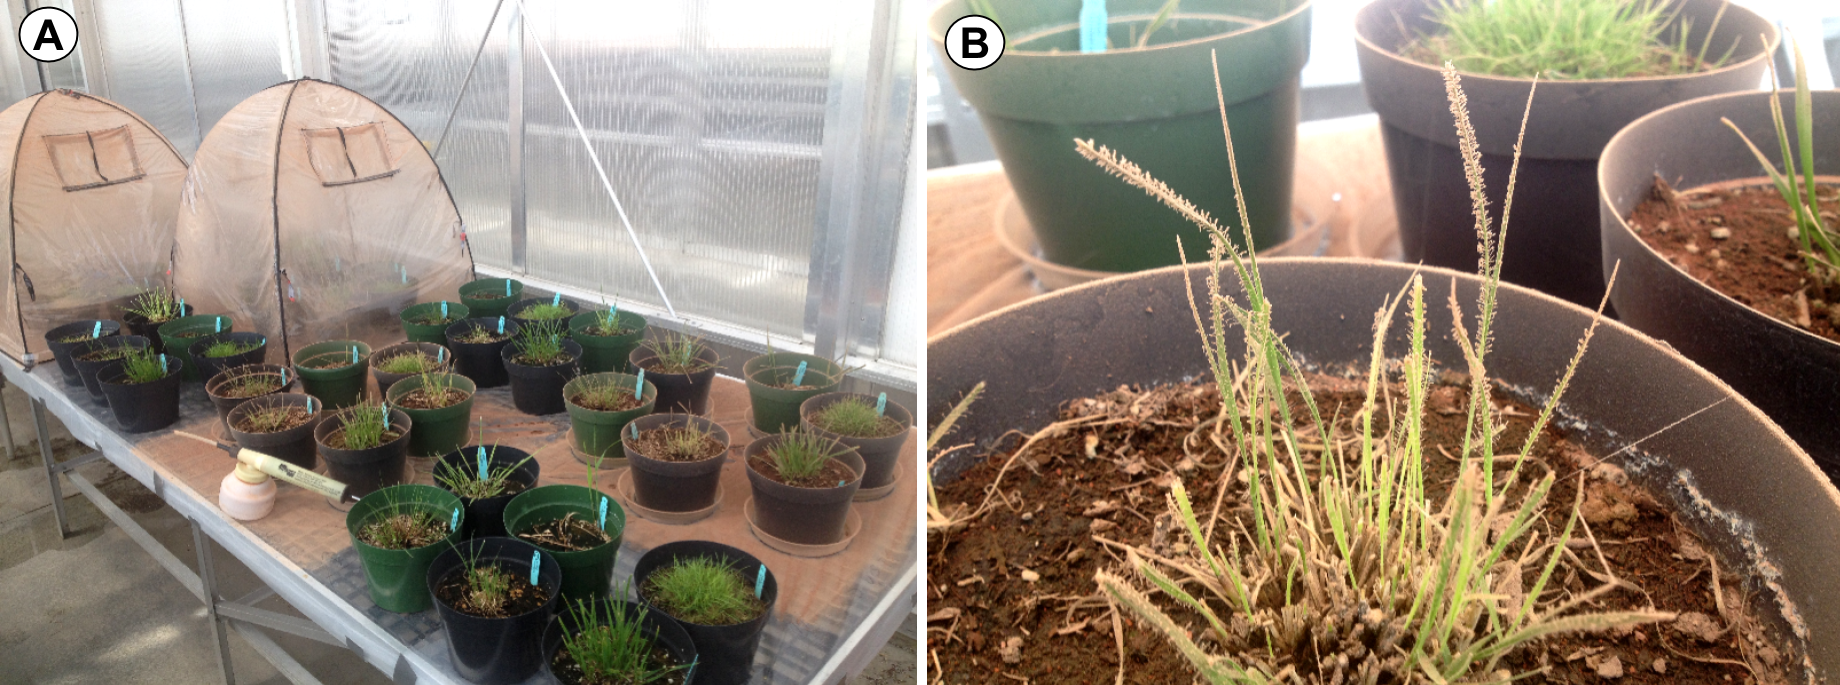
\includegraphics[width=\linewidth]{figures/GreenhouseDust}
  \caption{Applying dust to specific plants in the greenhouse. 
  \textbf{(A)} Perennial grasses were randomly assigned to six-pot groups in staggered dust or no-dust treatments. 
  Dust was applied via a hand-powered pump at the top of small vinyl greenhouse tents, and allowed 20 min to fully settle before a tent was lifted. 
  The same protocol was used for annual crops. 
  \textbf{(B)} Close-up of scoria road dust on leaf hairs of blue grama \emph{Bouteloua gracilis}. 
  \label{pic:dusting}}
\end{figure}

Dust treatments were designed to expose plants to very high dust levels similar to those measured along the most heavily-trafficked roads in the Bakken oil patch, where daily deposition rates averaged 2.83 g/m\textsuperscript{2}/day \citep{spiess2020}. 
In the greenhouse, each dust application event consisted of quickly pumping 40 g of dust into the tent and allowing 20 min to settle.
Annual crops received a dust application every other day for a 10-day period for a  a total dust exposure of 200 g/m\textsuperscript{2}.
Dust was applied to the perennial grasses every other day for a 14-day period for a total dust exposure of 280 g/m\textsuperscript{2}.

\subsection{Data collection} 

We measured five responses from the annual crops, which consisted of the following physiological measurements that are effective in determining plant responses to environmental stressors in controlled environments \citep{mcgranahan2018b}: 
\begin{enumerate}
	\item \emph{Stomatal conductance}\textemdash a measure of vapor flux through the leaf through stomata. 
	Greater flux can indicate susceptibility to moisture loss, and is one of the first responses to plant stress \citep{flexas2002}. 
	We used a clamp-style leaf porometer with a fixed diffusion path chamber (SC-1; METER formerly Decagon, Pullman, WA, USA). 
	\item \emph{Leaf temperature}\textemdash was recorded by the SC-1 leaf porometer for calculating stomatal conductance \citep{metergroup2020}. 
	We report leaf temperature here as it has been frequently been shown to increase following foliar dust deposition and is associated with stomatal closure \citep{eller1977, zia-khan2014}. 
	\item \emph{Chlorophyll content}\textemdash a measure of the plant's ability to assimilate carbon, grow, and produce fruit based on the density of photosynthetic pigments. 
	We used a chlorophyll content meter to measured chlorophyll content as the fluorescence emission ratio of light intensity at 735 nm/700 nm wavelengths
	 (CCM-300; Opti-Sciences, Inc, Hudson, NH, USA).
	\item \emph{Photosynthetic yield}\textemdash another measure of carbon assimilation efficiency, with a positive correlation with crop yield \citep{fischer1998}. 
	We report quantum yield of photosystem II ($\frac{F_{V}}{F_{M}}$;  \citet{kalaji2017}) as measured with an Opti-Sciences OS1p (Opti-Sciences, Inc, Hudson, NH, USA). 
	\item \emph{Specific leaf area}\textemdash is calculated as the dry mass of a leaf divided by its leaf area and is a measure of plant tissue available for photosynthesis and gas exchange. 
	We used the first three most-developed leaves at the top of each plant. 
	Leaf area was measured with a bench-mounted leaf area meter (LI-3000C \& LI-3050C; LI-COR, Inc, Lincoln, NE, USA), and dry mass determined by placing each leaf in paper envelopes and dried at 60\textsuperscript{o}C for 48 hrs and weighed.
	Because this is a destructive response, data are limited to only one sampling event per pot.
\end{enumerate} 

For each dust application event, non-destructive physiological measurements were made before and after dusting to determine short-term responses to foliar dust deposition. 
Approximately two hours passed between samples.
Care was taken to disturb as little foliar dust as possible.
Each subsequent sampling event measured the plants' responses to an increasing level of dust exposure\textemdash the most-recent dusting + all dust remaining from previous dustings. 
As a destructive measurement, specific leaf area was only determined at the end of the study. 

The singular response recorded from perennial grasses was aboveground biomass recovery following clipping. 
After an initial clipping to determine pre-treatment biomass, each pot was clipped twice more, each following 7 dusting events. 
All plant matter within 1 cm of soil surface was clipped, placed in paper envelopes, and dried at 60\textsuperscript{o}C for 48 h before weighing.
We expressed biomass recovery proportionally, as a percentage of the initial pre-treatment clipping. 

\subsection{Data analysis}

After ensuring all response variables followed a normal distribution, we fit linear mixed-effect models with the \texttt{lmer} function from the \emph{lme4} package in the \textsf{R} statistical environment \citep{bates2015, rcoreteam2019}. 
We employed a statistical framework developed for the analysis of plant trait and growth recovery data from controlled environmental conditions that emphases regression coefficients and associated confidence intervals as measures of effect size \citep{rinella2010,mcgranahan2018, mcgranahan2018b}. 
Model development followed \citet{cheng2010}'s principles of ``good enough'' longitudinal mixed models that control for known primary sources of variation in the experimental design. 
In our models, known sources of random variation included blocks, rounds, and repeated measures of individual pots. 
Models were fit for each measurement, which served as dependent response variables. 
Normality of residual error of all models was also confirmed. 
Data and script for analysis are in the Supplemental Information. 

For annual crops, we conducted two sets of analyses comparing short-term and long-term responses. 
To test the immediate effect of foliar dust deposition on annual crop physiological responses, we subtracted pre-dusting values from post-dusting values for each pot (mean of three leaves/plant)  and used this difference as the dependent variable in linear mixed-effect regression models. 
For species-level analysis, models were fit for each response with species as fixed effect and the intercept term removed to test whether the dust response for each species differed from zero; block, dust application event, and pot were fit as random effects. 
For an overall analysis of short-term dust impacts on physiology, we fit response as a fixed effect and removed the intercept term, and fit block, round, species, and pot as random effects. 
To facilitate comparison of effect sizes on a common scale, regression coefficients were centered and scaled by dividing centered columns by their standard deviation using \texttt{scale}. 
95\% confidence intervals were extracted for each fixed effect with \texttt{lme4::fixef} and \texttt{confint}. 
 
To test the long-term effect of dust accumulation throughout the study, we compared dusted and undusted plants across all sampling periods. 
Fixed effects consisted of two categorical predictor variables: dust treatment and plant species. 
The independent variables included dust exposure (dusted or undusted) and the interaction between species and dust exposure; removing the intercept term allowed these interaction terms to test species-specific dust effects along with the overall (average) dust effect. 
For repeated non-destructive treatments, random effects included block, sampling event, and pot; for the single specific leaf area data, the random effect included only block.
Models for each response were compared against a null model via analysis of deviance. 
Scaled regression coefficients and 95\% confidence intervals were extracted for the overall dust effect and each species' interaction with dust exposure as above. 

We employed a similar modelling and parameter estimation approach for perennial grass biomass recovery, except we compared several alternative models using an information-theoretic model selection approach. 
In addition to the dust exposure + species x dust interaction and null models described above, we also compared a model in which the species term was replaced with a term for photosynthetic pathway (C\textsubscript{3} vs. C\textsubscript{4}) to test for common responses by functional group. 
These three models were ranked according to their AIC\textsubscript{c} values using the \texttt{aicctab} function in the \textsf{R} package \emph{AICcmodavg} \citep{mazerolle2016}. 

\section{Results} 

Statistical results of regression modelling are presented here as effect sizes estimated from regression coefficients and 95\% confidence intervals. 
Mean and standard error for each response by sampling event and species are presented in Supplemental Information. 

\subsection{Annual crops}

\subsubsection{Short-term responses}

Short-term responses to foliar dust application were only apparent in chlorophyll concentration, which tended to increase after dusting for all species (Fig.~\ref{fig:st_cropCIs}). 
Stomatal conductance readings were slightly higher for barley and wheat, declined in pinto bean and sunflower, and were highly variable for maize, sorghum, and lentil. 
Photosynthetic yield was equally variable, with non-zero reductions in maize and lentil and a negative trend for sorghum. 
Pinto beans and sunflowers had substantial enough increases to drive an The overall non-zero increase in photosynthetic yield was driven by substantial increases in pinto beans and sunflowers. 
Leaf temperature was variable among species such that there was no overall significant difference from zero, but there were non-zero reductions in leaf temperature for wheat and sorghum.  

\begin{figure}
	%\centering
	 \hspace{0.5em}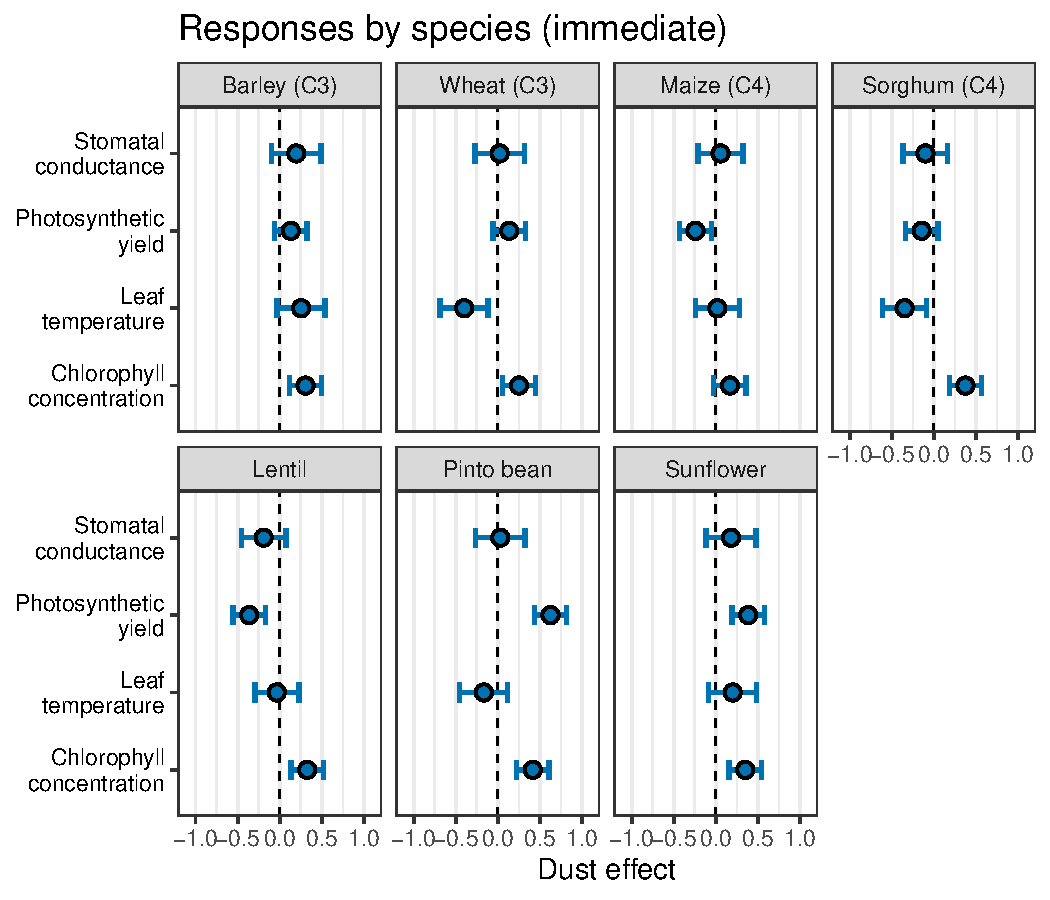
\includegraphics[width=0.8\linewidth]{figures/st_spp_gg-1}
	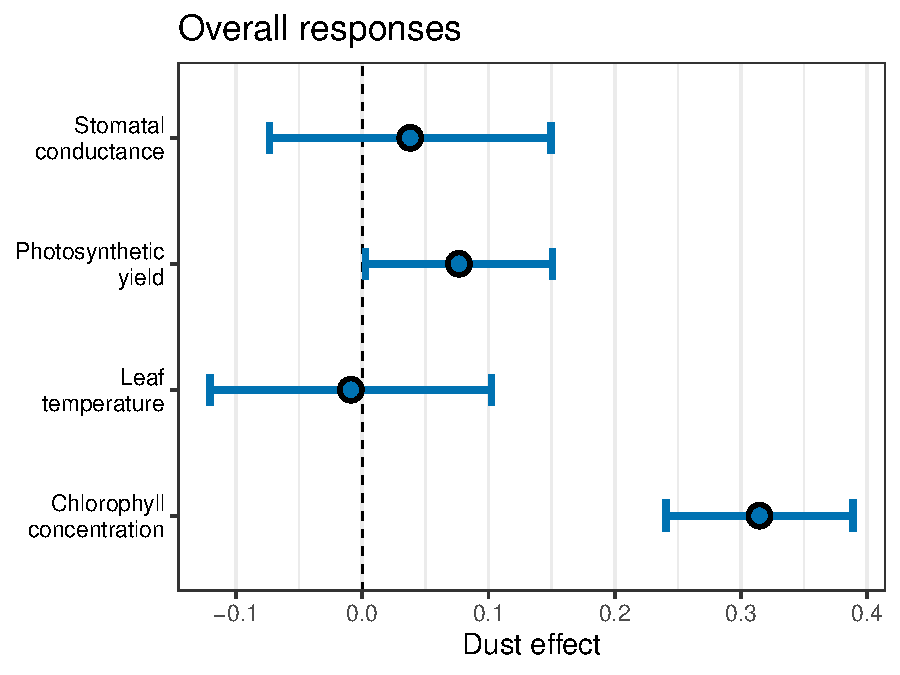
\includegraphics[width=0.75\linewidth]{figures/st_ov_gg-1}
	\caption{Short-term effects of dust exposure on annual crop physiology and leaf temperature by species (Top) and by response averaged across all species (Bottom).
		Approximately two hours passed between pre-dusting and post-dusting readings. 
		When 95\% confidence intervals do not overlap zero, dust exposure had an effect equal to the magnitude and sign of the plotted point; when 95\% confidence intervals do overlap zero, dust exposure had no effect on the measured response. \label{fig:st_cropCIs} }
\end{figure}

\subsubsection{Long-term responses}

When dusted plants were compared to undusted plants over the duration of the study, mixed-effect regression models for each response fit with species and dust terms explained variation better than null models (Table~\ref{tab:cropAIC}). 
Highly-ranked models with dust-species interaction terms for chlorophyll concentration, leaf temperature, and photosynthetic yield indicate that responses were quite variable among species. 

At the species level, photosynthetic yield tended to show meaningful (non-zero) increases among grasses (maize, wheat, and sorghum), but only sorghum showed a meaningful increase in chlorophyll content, as well (Fig.~\ref{fig:lt_cropCIs}). 
Leaf temperature was highly variable across species\textemdash maize, sorghum, and lentil showed strong declines in leaf temperature of dusted plants vs. undusted over the duration of the study; wheat, pinto bean, and sunflower showed no meaningful difference in leaf temperature, and barley tended to increase. 
For all other measures, 95\% confidence intervals overlapped zero, indicating no meaningful response to dust exposure. 

Averaged across all species over the duration of the study, chlorophyll content and photosynthetic yield were greater and stomatal conductance lower among dusted plants (Fig.~\ref{fig:lt_cropCIs}). 


\begin{table}[!h]
\centering
\begin{tabular}{llrrrrr}
  \hline
Response & Model & K & AICc & $\Delta$AICc & AICcWt & Cum.Wt \\ 
  \hline
Chlorophyll concentration & species x dust & 16 & 4023.2 & 0.0 & 0.80 & 0.80 \\ 
   & species + dust & 10 & 4026.0 & 2.8 & 0.20 & 1.00 \\ 
   & species & 9 & 4140.6 & 117.4 & 0.00 & 1.00 \\ 
   & dust & 4 & 4656.6 & 633.4 & 0.00 & 1.00 \\ 
   & null (Intercept only) & 3 & 4683.7 & 660.5 & 0.00 & 1.00 \\ 
  Stomatal conductance & species + dust & 10 & 83.6 & 0.0 & 0.80 & 0.80 \\ 
   & species x dust & 16 & 86.7 & 3.1 & 0.17 & 0.97 \\ 
   & species & 9 & 90.3 & 6.7 & 0.03 & 1.00 \\ 
   & dust & 4 & 1122.6 & 1039.0 & 0.00 & 1.00 \\ 
   & null (Intercept only) & 3 & 1127.9 & 1044.3 & 0.00 & 1.00 \\ 
  Leaf temperature & species x dust & 16 & 2552.7 & 0.0 & 1.00 & 1.00 \\ 
   & species & 9 & 2668.7 & 116.0 & 0.00 & 1.00 \\ 
   & species + dust & 10 & 2668.9 & 116.2 & 0.00 & 1.00 \\ 
   & null (Intercept only) & 3 & 2729.3 & 176.6 & 0.00 & 1.00 \\ 
   & dust & 4 & 2729.8 & 177.1 & 0.00 & 1.00 \\ 
  Photosynthetic yield & species x dust & 16 & 3627.5 & 0.0 & 1.00 & 1.00 \\ 
   & species + dust & 10 & 3669.0 & 41.5 & 0.00 & 1.00 \\ 
   & species & 9 & 3701.6 & 74.1 & 0.00 & 1.00 \\ 
   & dust & 4 & 4749.1 & 1121.5 & 0.00 & 1.00 \\ 
   & null (Intercept only) & 3 & 4769.8 & 1142.3 & 0.00 & 1.00 \\ 
  Specific leaf area & species & 9 & 1798.7 & 0.0 & 0.69 & 0.69 \\ 
   & species + dust & 10 & 1800.4 & 1.8 & 0.28 & 0.97 \\ 
   & species x dust & 16 & 1805.0 & 6.4 & 0.03 & 1.00 \\ 
   & null (Intercept only) & 3 & 1909.2 & 110.5 & 0.00 & 1.00 \\ 
   & dust & 4 & 1911.1 & 112.4 & 0.00 & 1.00 \\ 
   \hline
\end{tabular}
\caption{Results of AICc-based ranking of linear mixed-effect regression models comparing four physiological responses + leaf temperature by species, dust application, an additive multiple-regression model, and a multiple regression model with an interaction term, against a null, intercept-only model.} 
\label{tab:cropAIC}
\end{table}
 

\begin{figure}
	%\centering
	 \hspace{0.5em}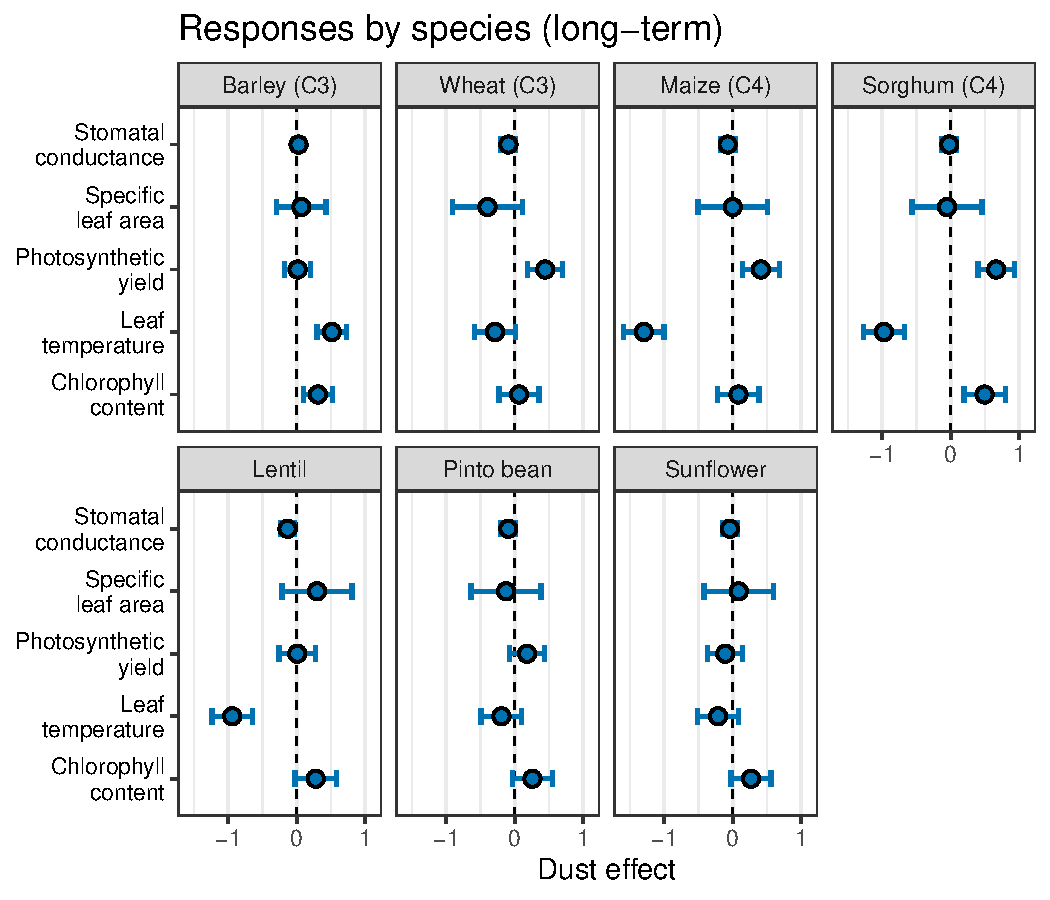
\includegraphics[width=0.8\linewidth]{figures/lt_spp_gg-1}
	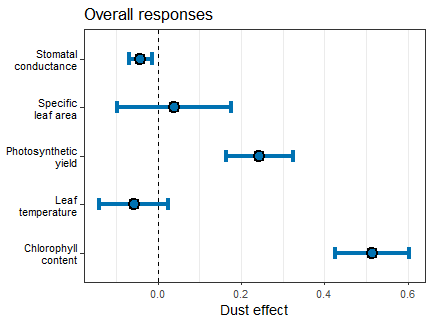
\includegraphics[width=0.75\linewidth]{figures/lt_ov_gg-1}
  \caption{Effect of dust exposure on annual crop physiology and leaf temperature by species (Top) and by response averaged across all species (Bottom). 
  	When 95\% confidence intervals do not overlap zero, dust exposure had an effect equal to the magnitude and sign of the plotted point; when 95\% confidence intervals do overlap zero, dust exposure had no effect on the measured response. \label{fig:lt_cropCIs} }
\end{figure}

\subsection{Perennial grasses} 

The mixed-effect regression model testing for species-specific responses to dust exposure was much more explanatory of variation in biomass recovery than responses grouped by photosynthetic pathway (Table~\ref{tab:grassAIC}).
There was no consistent effect of dust exposure among perennial grass recovery following repeated defoliation (Fig.~\ref{fig:grassCIs}). 
The average dust effect was negative, but not different than zero. 
Tall fescue was the only species to show a non-zero response, in which pots exposed to dust actually grew back more biomass after clipping than those not exposed to dust. 

\begin{table}[ht]
\centering
\begin{tabular}{lrrrrrrr}
  \hline
Model & K & AICc & $\Delta$AICc & ModelLik & AICcWt & LL & Cum.Wt \\ 
  \hline
species x dust & 18.0 & -197.0 & 0.0 & 1.0 & 1.0 & 117.9 & 1.0 \\ 
  C3/C4 x dust & 6.0 & -85.3 & 111.7 & 0.0 & 0.0 & 48.8 & 1.0 \\ 
  null (Intercept only) & 3.0 & -84.4 & 112.6 & 0.0 & 0.0 & 45.2 & 1.0 \\ 
  Dust exposure & 4.0 & -82.5 & 114.4 & 0.0 & 0.0 & 45.4 & 1.0 \\ 
   \hline
\end{tabular}
\caption{Results of AICc-based ranking of linear mixed-effect regression models comparing perennial grass biomass recovery by species, dust application, photosynthetic pathway (C3/C4), interactions between these variables, and a null, intercept-only model.} 
\label{tab:grassAIC}
\end{table}
 

\begin{figure}
	\centering
	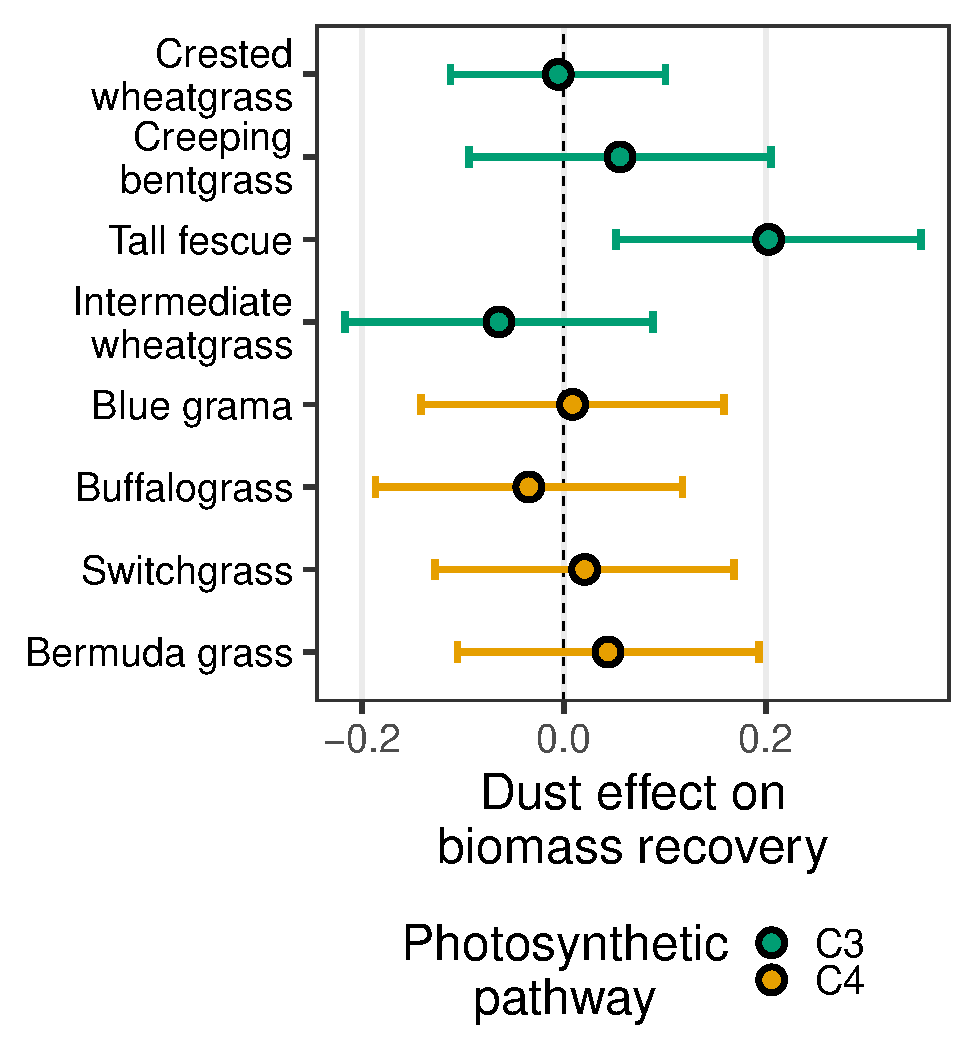
\includegraphics[width=0.6\linewidth]{figures/GrassCIs-1}
	\caption{Effect of dust exposure on perennial grass recovery following two clipping events, by species and photosynthetic pathway. 
		The average response across all species is plotted below the species-specific responses.
		When 95\% confidence intervals do not overlap zero, dust exposure had an effect equal to the magnitude and sign of the plotted point; when 95\% confidence intervals do overlap zero, dust exposure had no effect on the measured response. \label{fig:grassCIs} }
\end{figure}


\clearpage 

\section{Discussion} 

The ecology of dust has received little attention, due likely to the study of aeolian processes falling mostly in the geosciences. 
But desertification, land use intensification, and development of unconventional and alternative energy sources are expected to increase fugitive dust emissions in ecosystems worldwide, with largely unknown ecological consequences \citep{field2010}.  
However, most work at the intersection of vegetation and dust focuses on dust generation, rather than the impacts of deposition \citep[e.g.,][]{belnap2014, flagg2014,nandintsetseg2015}. 

Our data indicate that exposure to extremely high levels of road dust affects physiological parameters related to growth and productivity in annual crops, especially as foliar dust load accumulates. 
Chlorophyll concentration tended to increase in all annual plants within 1-2 hours of dust exposure, which remained high (along with photosynthetic yield) over the duration of the study, whereas stomatal conductance tended to decrease over the two-week study period.
Conversely, we found little evidence that high levels of dust reduces the ability of perennial grasses to recover from repeated defoliation, regardless of photosynthetic pathway or functional group. 

Two novel components of this study include the analysis of responses to both immediate exposure to dust deposition and dust accumulation over the duration of the study, and the extremely high levels of dust to which plants were exposed. 
For example, \citet{bao2015} exposed plants up to a maximum of 16.64 g/m\textsuperscript{2} of dust, and \citet{thompson1984} tested plants at dust concentrations of 5\textendash 10 g/m\textsuperscript{2}, having only measured foliar dust loads of 2 g/m\textsuperscript{2} in the environment. 
\citet{matsuki2016} reported plants along roadways were exposed to 20\textendash 70 g/m\textsuperscript{2} per month, or 0.67\textendash 2.3 g/m\textsuperscript{2} per day, which is still below the average daily deposition rate within the road effect zone along heavily-trafficked, unpaved roads in the Bakken oil patch (2.8 g/m\textsuperscript{2}). 
To simulate the cumulative effect of such heavy dust deposition, by the end of our dusting study, plants had been exposed to 200\textendash 280 g/m\textsuperscript{2}.

While we did expect to see dust accumulation leading to lower stomatal conductance, we did not expect the trend towards lower leaf temperatures and higher values of responses related to photosynthetic activity among dusted annual crops. 
Previously-reported effects of foliar dust deposition include reduced chlorophyll concentration, increased temperature of leaves and the canopy, and reduced efficiency of plant processes \citep{eller1977, ulrichs2008,zia-khan2014, sarma2017}. 
While photosynthetic activity might have increase to compensate for reduced efficiency, we did not observe differences in leaf temperature as recorded by our instruments (data not shown). 
Foliar dust can also increase the reflectance of light in the visible spectrum \citep{wu2016}, which could have a cooling effect on leaves. 
Dust can also create a diffusive, light-scattering effect that reduced photoinhibition at high levels of sun exposure, which has been shown to increase gas exchange and improve photosynthesis in economic plants \citep{jifon2003, kromdijk2016}. 
Whether reflectance or light-scattering occurs in a high-sunlight field situation, or if either effect of foliar dust deposition could actually translate to improved plant performance, is unknown. 

Thus, an obvious caveat is the fact that this study was conducted under the ideal growth conditions of a greenhouse. 
Plants subject to environmental stressors (e.g., heat, drought, insects) in the field might be more susceptible to foliar dust load as a compounding factor. 
On the other hand, environmental stressors might simply have a much greater magnitude of impact on plant condition \citep{matsuki2016}. 
Furthermore, we did not track plants to maturity and reproduction\textemdash barriers to pollination in such a study would preclude meaningful yield data\textemdash but the physiological responses we measured have been correlated with biomass production and crop yield \citep[e.g.,][]{fischer1998, zia-khan2014}. 
And although we only measured the recovery of perennial grasses to defoliation, our results are relevant indicators of potential in-situ dust response because perennial grasses like those in this study rarely rely on seeds for reproduction. 
For example, fewer than 1\% of prairie grass ramets are seedlings \citep{benson2006}. 
 
While we have no certain explanation for why tall fescue recovered more biomass after clipping when exposed to dust, we attribute it at least in part to a potentially novel benefit derived from the symbiotic relationship with a fungal endophyte. 
The benefits conferred by epichloae endophytes to host grasses have been widely documented, and include increased tolerance of heat and drought stress \cite{gibert2012,he2013}. 
Epichloae infection has been shown to increase biomass production under drought stress in the related Arizona fescue \emph{Festuca arizonica} \citep{morse2002}; further work should test the role of endophyte infection as a modulator of host plant response to foliar dust deposition. 

Chemical impacts, via both contact with plant tissues and altered soil chemistry, must also be considered. 
Dust certainly re-distributes nutrients and leads to increased concentrations where dust settles and accumulates \citep{brahney2014, lawrence2010}. 
The scoria used to surface unpaved roads in the Bakken has a lava-like nature, having been ``formed by the baking of the clay or shale immediately above the lignite seam \citep[][p.435]{roe1950}'' and is likely relatively inert. 
Other studies of particulate impacts on plants have included urban pollution \citep{bao2015} and limestone \citep{brown2009, organiscak2004}, which can alter vegetation composition through calcium deposition and soil pH changes. 
\citet{armbrust1986} specifically noted that physical damage or toxicity was not necessary to reduce photosynthetic activity in crops affected by wind-blown dust, but advised that wind and rain would keep foliar accumulation below critical levels. 
Increased traffic due to expanded energy development might change that.

As stated above, the ecological consequences of the anthropogenic processes that drive dust emissions and the  aeolian processes that transport and deposit fugitive dust are poorly understood, but are receiving more attention \citep{field2010}. 
As such, the ecological implications of the results demonstrated here are equally unclear, although the unexpected direction of some responses in this greenhouse trial merit extension to longer-term field experiments. 

We suggest three scales of ecological impacts of dust deposition and accumulation: At the finest scale, the physiology of individual plants is clearly affected by dust at very short (hourly) and short (weekly) time frames, sometimes counter-intuitively. 
These effects likely scale up to variability in plant productivity and competitiveness to effect changes in community composition that are likely modulated by dust-driven changes in soil chemistry. 
More broadly, there is increasing evidence that dust affects plant-animal interactions, which might mean dust deposition can affect not only community composition but ecosystem service delivery. 
For example, dust has been shown to interfere with pollen-stigma interactions and fruit set in several species of plants, but the overall effect on individual fitness is not clear \citep{waser2016, zhang2019}. 


\paragraph{Acknowledgements}
This work was supported by National Institute of Food and Agriculture Hatch Project 1009910, North Dakota State University Office of the President, and the North Dakota State Agricultural Experiment Station.
Jonathan Spiess and Jennifer Foggia provided technical assistance. 
Aaron Daigh and Craig Whippo contributed to field studies that prompted this investigation.
Mark Brunson inspired the study design.

\paragraph{Supplemental Information}

Supplemental information is available at the online version of this paper:

\textbf{S1} Plots of summarised data and \textsf{R} script.
Plant data for analysis is attached in the \texttt{.pdf} as an \textsf{R} workspace.

\paragraph{Compliance with Ethical Standards}
This paper complies with all relevant ethical standards. 

\bibliographystyle{spbasic}      
\bibliography{GreenhouseDust} 




\end{document}